\chapter{Spectral Analysis}
\label{ch:spettro}
A fundamental aspect of the Plasma Coagulation Controller is what species are produced and deposited during its application. Various studies observed the spectrum of plasma DBD discharge in air at atmosferic pressure and ambient temperature (\cite{DBDair_Trot}, \cite{DBDAirTypicalSpec}), meanly it presents peaks relative to reactive species from water, oxygen, nitrogen and its oxides at visible wavelenght, from $\num{200}$ to $\SI{880}{\nano\meter}$.

We are intersted in plasma that contains molecules involved in blood coagulation mechanisms, Reactive Oxidant Species (such as hydroxil radical \ce{OH}) and Reactive Nitrogen Species (derived from nitric oxide \ce{NO}) (\cite{6153386}). In this spectroscopy study is given particular attention to them and their precursor, i.e. the presence of transitions relative to hydroxil, oxygen and molecular nitrogen.


\section{Radiation emission}
As remembered in previous chapters, at the exit of source head is produced plasma from a mixture gas of helium or argon and air, so there is a certain fraction of free charges inside the plume fo plasma. Along free electrons, there are ions and species that colliding with them are in an excited state, metastable or with small lifetime. All those reactive species partecipe in different reactions, and also in excitation and de-excitation reactions with conseguent emission of radiation. When an electron goes from state p at higher energy to state k of lower energy, is emitted radiation with central wavelenght $\lambda_0$. Power emitted by this radiation is given by radiant flux $d\phi_{\lambda}$ and selecting a solid angle as in figure, is possible to define radiance $L_{\lambda}$, and intensity $I$, as in equations \ref{eq:emission}. Intensity for a radiation ultimately depends on $n(p)$, population density for state p, and Einstein Coefficient for the transition $A_{pk}$ that is typical for the transition (\cite{book:291477}).

\begin{minipage}{.48\textwidth}
 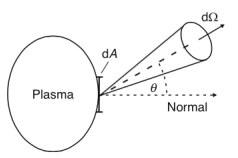
\includegraphics[width=0.8\textwidth]{Images/Spectroscopy/plasmaemission.png}
\end{minipage}
\begin{minipage}{.48\textwidth}
\begin{equation}
 \begin{split}
 &\lambda_{0} = \frac{hc}{E_p - E_k} \\
 &L_{\lambda} = \frac{d^2\phi_{\lambda}}{dA \cos(\theta) d\Omega} \\
 &I = \int L_{\lambda} d\lambda = n(p) A_{pk}
 \end{split} 
 \label{eq:emission}
\end{equation}
\end{minipage}


Using air as gas, composed by molecules, at visible wavelenght are observed vibronic transitions where molecule goes from a vibrational state to another, with a change of vibrational quantum number $\nu$, and/or from a rotational state to another, with change of quantum number $J$ (\cite{book:137793}, \cite{wiki:vibronic}). When there is a vibrational transition, each line corresponds to different numbers $\nu'-\nu''$, these are transitions well spaced in the spectrum, easy to recognize. Rotational transitions gives birth to bands of little-spaced peaks hard to resolve whitout an efficient spectrometer.

There are many reactions involving oxygen and nitrogen (see for example \cite{Kossyi_1992}), in this study we determine only principal transition observable with our spectrometer, to know dominant reactive species present in our plasma plume.


\section{Experimental setup}
For the source it's used a prototype that presents electrical specifics and settings same as source A described in previous chapters. A metal plate is positioned as target at a distance of $\SI{10}{\milli\meter}$ from plasma exit. To ignite plasma is used helium, with flow set to $\SI{2}{\liter/\minute}$.
To measure emission it's used a spectrometer IsoPlane, that thanks to diffraction separates emissions with different wavelenghts using a plane grating. The spectrometer has a focal lenght of $\SI{320}{\milli\meter}$ and is equipped with three different gratings: $\num{150}$, $\num{1200}$ and \SI{2400}{gg/\milli\meter}, corresponding to different resolutions of $\num{0.26}$, $\num{0.03}$ and $\SI{0.01}{\nano\meter}$.
As in figure \ref{fig:app}, light emitted by plasma is collected with a quartz lens %...
and passes trough an optical fiber %..
connected to the spectrometer entry, while at the spectrometer exit there is a CCD camera of $2048$ pixels and a count limit of $\num{65000}$.
\begin{figure}
\centering
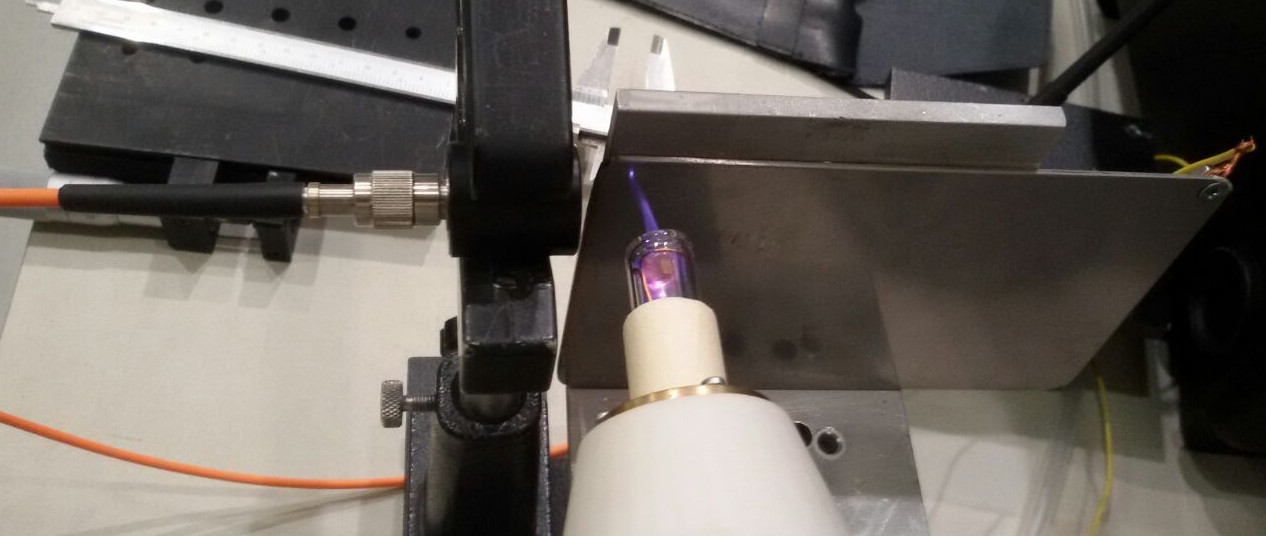
\includegraphics[width=.6\textwidth]{Images/Spectroscopy/apparato.jpg}
\caption{Setup of the experiment: there is the working source, the metal target and the optical setup on the left.}
\label{fig:app}
\end{figure}

Once a grating is chosen, the acquisition system can be set at a starting wavelenght and from there it takes measures until the end of the CCD, so for a wavelenght interval different for different gratings.
For every measure is selected an appropriate acquisition time that permits to observe peaks with a good count number and avoid saturation.

It's important to stress out that, with this measuring method and due to complexity of plasma reactions and composition, it's not possible to extrapolate quantitative considerations between different species concentration. However it's possible to recognize the presence of certain species and make some considerations watching spectra variation with different experimental setup.

An intersting parameter is the working distance between source's head and target, so we observe spectra focalizing the lens in two different positions:
\begin{itemize}
 \item position 1: as close as possible to plasma exit point
 \item position 2: close to the target, at \SI{10}{\milli\meter} from plasma exit point
\end{itemize}

Reactions that produce and recombine reactive species, and consequently density and lifetime of species, are influenced by electric field and duration of the discharge. We observe spectra changing amplitude and frequency of the pulse, with tree different combinations that corresponds to different power coupled with the discharge:
\begin{itemize}
 \item low: $f = \SI{5}{\kilo\hertz}$ and $\Delta t = \SI{15}{\micro\second}$
 \item medium: $f = \SI{10}{\kilo\hertz}$ and $\Delta t = \SI{10}{\micro\second}$
 \item high : $f = \SI{15}{\kilo\hertz}$ and $\Delta t = \SI{10}{\micro\second}$
\end{itemize}


\section{Line recognition}
To see what's generally produced in a discharge is taken a spectrum for the entire wavelenght's region intersted, from $\num{230}$ to $\SI{800}{\nano\meter}$, with standard setup of medium power and position 1.
First is made a rapid acquisition with the lowest resolution possible, to see intersting regions and have an idea of required exposition times. After that is made a slow acquisition with higher resolution for all wavelenghts. The entire spectrum is reconstructed attaching different spectra, showed in figure \ref{fig:spectr}, where are labelled principal transitions.
For every measure is taken also a background spectrum, without plasma, to recognize peaks that are not from the plasma.

Data is read with IDL routines (\cite{}) and analyzed with ROOT TSpectrum.h library (\cite{}). Every spectrum is divided by its exposition time, to normalize different measures. Then is estimated the white noise contribution as mean value from a portion of the spectrum that doesn't presents peaks and its subtracted to the counts for each wavelenght. Peaks are then found with TSpectrum functions (where is possible to set a treshold in heigth and the general width for lines to be searched) and peaks from background are isolated in plasma spectra. Definitive position for each transition is found with a gaussian fit in an interval that takes into consideration the asymmetry where it's needed.

As said before, this study is focused on measure related to ROS and NRS, so in lines for \ce{NO}, \ce{OH} and \ce{N_2}.

\begin{figure}
\centering
\includegraphics[width=0.99\textwidth]{Images/Spectroscopy/spettrotot_unico_label_def.png}
\caption{Spectrum with an helium flow of $\SI{2}{\liter/\minute}$, pulse parameters of $f = \SI{5}{\kilo\hertz}$ and $\Delta t = \SI{16}{\micro\second}$, optical position $1$, near plasma exit}
\label{fig:spectr}
\end{figure}


\paragraph{\ce{NO} lines}
Are observed two doublets for the transition \ce{A^2\Sigma^+ - X^2\Pi} with vibrational numbers (0-0) and (0-1) (\cite{Knie:166349}, \cite{VANSPRANG197955}), presented in table \ref{tab:spettroNO}. Intensities for the peaks are normalized with maximum value of $\num{1000}$ for the acquisition, the table shows as the intensities for this transition is very low. Other transition relative to this molecule have even lower relative intensity and are not observed in our study.
\begin{table}[h]
\centering
 \begin{tabular}{cc}
  \toprule
  $\lambda$ \text{[}\si{\nano\meter}\text{]} &\text{I [arb.u.]}\\
  \midrule
  \num{236.31(24)}  &27\\
  \num{237.00(15)}  &26\\
  \num{247.02(5)}  &28\\
  \num{247.86(12)}  &27\\
  \bottomrule
 \end{tabular}
 \caption{Peaks measured for \ce{NO}.}
 \label{tab:spettroNO}
\end{table}


\paragraph{\ce{OH} lines}
Is observed the rotational band for transition (\ce{A^2\Sigma}, $\nu' = 0$ $\rightarrow$ \ce{X^2\Pi}, $\nu'' = 0$), observing $13$ principal lines (\cite{doi:10.1142/S0129183100000857}).
In figure \ref{fig:OHsp} a zoom on the spectrum, in table \ref{tab:sptrOH} peak values.
\begin{figure}
 \centering
 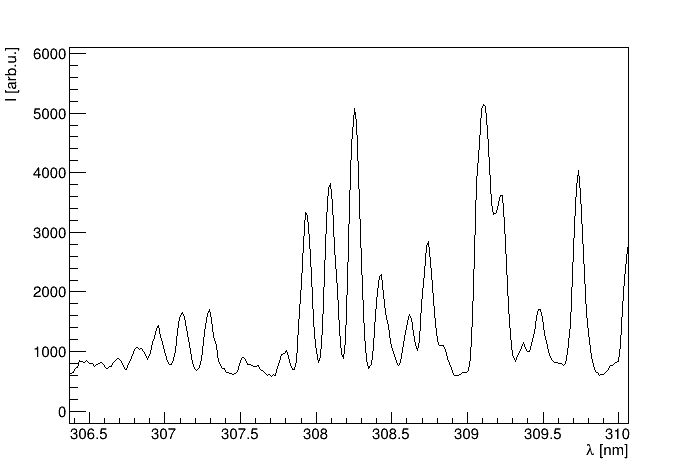
\includegraphics[width=0.6\textwidth]{Images/Spectroscopy/OH_f5t16v.png}
 \caption{Zoom for OH peaks}
 \label{fig:OHsp}
\end{figure}
\begin{table}
 \centering
 \begin{tabular}{cc}
  \toprule
  $\lambda$ \text{[}\si{\nano\meter}\text{]} &\text{I [arb.u.]}\\
  \midrule
  \num{306.96(1)}  &53\\
  \num{307.11(1)}  &58\\
  \num{307.29(1)}  &62\\
  \midrule                          
  \num{307.94(1)}  &142\\
  \num{308.09(1)}  &148\\
  \num{308.26(1)}  &161\\
  \num{308.43(1)}  &112\\
  \num{308.62(1)}  &46\\
  \num{308.74(1)}  &137\\
  \midrule                          
  \num{309.11(1)}  &151\\
  \num{309.22(1)}  &120\\
  \num{309.45(1)}  &36\\
  \num{309.73(1)}  &125\\
  \bottomrule
 \end{tabular}
 \caption{Peaks measured for \ce{OH}.}
 \label{tab:sptrOH}
\end{table}


\paragraph{\ce{N_2} and \ce{N+_2} lines}
Measured spectrum presents several lines for diatomic molecule dinitrogen, including strongest lines. Is observed the Second Positive System for \ce{N2} transition $\ce{C^3\Pi} \rightarrow \ce{B^3\Pi}$ and the First Negative System for \ce{N2+} transition $\ce{B^2\Sigma} \rightarrow \ce{X^2\Sigma}$, in table \ref{tab:sptrN} peak values (\cite{N2lab}, \cite{Britun_2007}). For \ce{N2} is found also a band of multiple rotational lines centered around \SI{336.58(1)}{\nano\meter}.
Some of the peaks are seen in the second diffraction order, where there is more distance between lines. In figure \ref{fig:N2} are presented two zooms for \ce{N2} lines.
\begin{figure}
 \centering
 \subfloat[Transitions with $\Delta \nu = 2$]{
    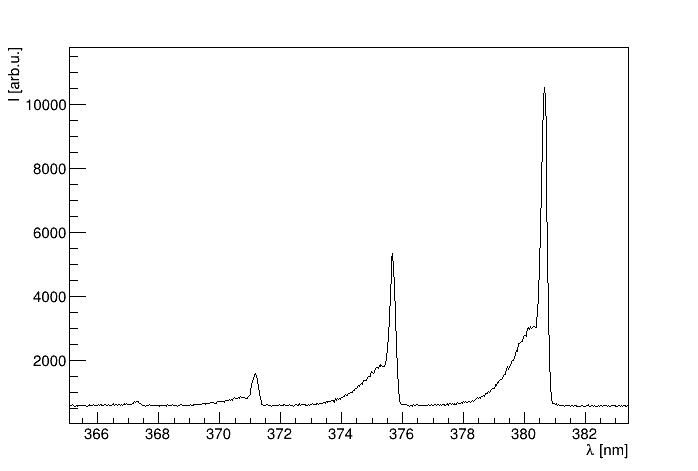
\includegraphics[width=0.45\textwidth]{Images/Spectroscopy/N2v_f5t16.png}
 }
 \hfill
 \subfloat[Strongest line (0-0)]{
    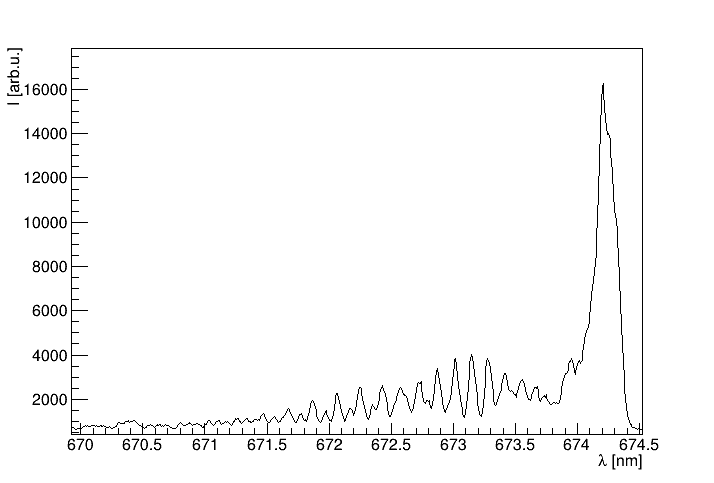
\includegraphics[width=0.45\textwidth]{Images/Spectroscopy/N2r_f5t16.png}
 }
 \caption{Zoom for \ce{N2} transitions.}
 \label{fig:N2}
\end{figure}

\begin{table}
\centering
 \begin{tabular}{cccc}
  \toprule
                            &$\lambda$ \text{[}\si{\nano\meter}\text{]} &\text{I [arb.u.]}  &($\nu'-\nu''$)\\
  \midrule
  \multirow{3}*{\ce{N_2}}   &\num{316.03(1)}  &381  &(1-0)\\
                            &\num{337.11(1)}  &1000 &(0-0)\\
                            &\num{357.77(1)}  &722  &(0-1)\\
  \midrule
  \multirow{4}*{\ce{N_2}}   &\num{367.22(20)}  &58  &(3-5)\\
                            &\num{371.12(4)}  &172  &(2-4)\\
                            &\num{375.66(2)}  &232  &(1-3)\\
                            &\num{380.64(2)}  &423  &(0-2)\\
  \midrule
  \multirow{2}*{\ce{N_2^+}} &\num{391.50(2)}  &355  &(0-0)\\
                            &\num{427.45(2)}  &180  &(0-1)\\
  \bottomrule
 \end{tabular}
 \caption{Peaks measured for \ce{N_2} and \ce{N+_2}.}
 \label{tab:sptrN}
\end{table}


\paragraph{Atomic lines}
Are observed other lines from elements present in the plume (\cite{NIST}):
\begin{itemize}
 \item \textbf{\ce{H_{\alpha}}} line corresponding to transition from quantum number $n=3$ to $n=2$
 \item \textbf{\ce{He}} two of the strongest lines for helium
 \item \textbf{\ce{O}} strong line of oxygen
\end{itemize}
\begin{table}
\centering
 \begin{tabular}{ccc}
  \toprule
                            &$\lambda$ \text{[}\si{\nano\meter}\text{]} &\text{I [arb.u.]}\\
  \midrule
  \ce{H_{\alpha}}           &\num{655.96(4)}  &113\\
  \midrule
  \multirow{2}*{\ce{He}}    &\num{586.94(5)}  &122\\
                            &\num{705.56(1)}  &649\\
  \midrule
  \ce{O}                    &\num{776.89(1)}  &393\\
  \bottomrule
 \end{tabular}
 \caption{Main peaks measured for other species found in plasma.}
 \label{tab:sptrother}
\end{table}



\section{Relative intensities}
It's studied spectra variation changing experimental setup: pulse settings and measurements position.
Intensities are evaluated for \ce{OH} and \ce{N2} species, collectively for the lines in a wavelength range specific for the peaks. For \ce{OH} lines is considered all the rotational band between $\num{306}$-\SI{309}{\nano\meter}, lines for \ce{N2} are separated in those between $\num{335}$-\SI{337}{\nano\meter} (rotational band and (0-0) transition) and those between $\num{368}$-\SI{382}{\nano\meter} (vibrational transitions with $\Delta \nu = 2$).

\paragraph{Pulse frequency} \ce{OH} lines for both positions have same intensity with low and medium power setup, while is lower with higher frequency, with similar behavior in both positions. \ce{N2} intensities also decrease with higher frequencies, for every lines, it reaches around $0.6\%$ for $f = \SI{15}{\kilo\hertz}$ in position 1, and lower values for position 2. It seems that production of those reactive species have rates dependant from pulse frequency, for high frequency there might be more relevant competitor reactions.

\paragraph{Sight position} At \SI{10}{\milli\meter} from the source, in position 2, intensities for \ce{OH} decreases drastically, under $0.1\%$ of values in position 1. \ce{OH} species seems to have small lifetime or mobility, so deposition of this species is higher when closer to the target.
For \ce{N2} intensities are equal at low frequency for both positions, while for higher frequencies they decrease more for position 2. For low frequency, concentration of excited \ce{N2} is high so even distant from the target we have high radiation emission. When it decreases, for higher frequencies, concentration lowers and we have few molecules that reach the target.
\begin{figure}
\centering
 \subfloat[\ce{OH} intensities in range $\num{306}$-\SI{309}{\nano\meter}]{
    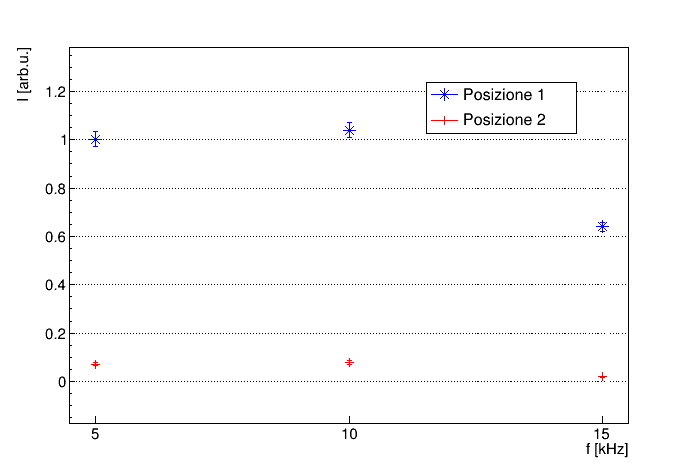
\includegraphics[width=0.48\textwidth]{Images/Spectroscopy/I_OH.png}
 }
 \hspace{0.55\textwidth}
 \subfloat[\ce{N2} intensities range $\num{335}$-\SI{337}{\nano\meter}]{
    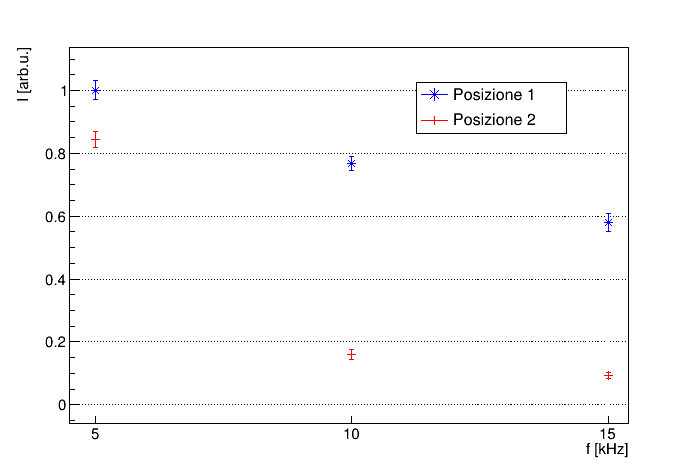
\includegraphics[width=0.48\textwidth]{Images/Spectroscopy/I_N2r.png}
 }
 \hfill
 \subfloat[\ce{N2} intensities range $\num{368}$-\SI{382}{\nano\meter}]{
    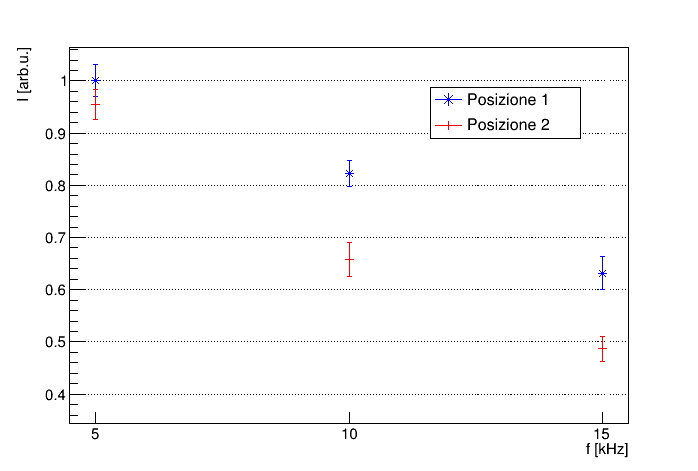
\includegraphics[width=0.48\textwidth]{Images/Spectroscopy/I_N2v.png}
 }
 \caption{Relative intensities in selected portions of the spectrum, for different frequencies, in blue for position 1 in red for position 2.}
 \label{fig:irel}
\end{figure}


\section{Estimation of plasma temperatures}
Possible to estimate plasma composition parameters. Rotational = temperature of ions, vibrational = storage energy. 
\subsection{Rotational temperature for \ce{OH}}
How, simulation, article.
\begin{figure}
\centering
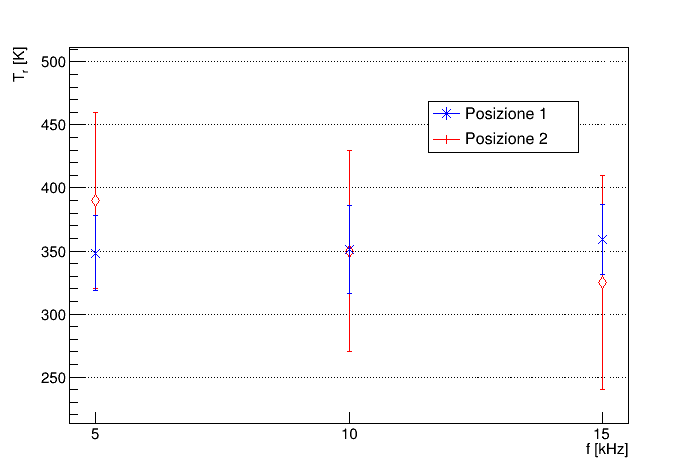
\includegraphics[width=0.65\textwidth]{Images/Spectroscopy/TrOH.png}
 \caption{Estimation of rotational temperature of \ce{OH} molecule, for different frequencies, in blue position 1 in red position 2.}
 \label{fig:TrOH}
\end{figure}

\subsection{Rotational temperature for \ce{N_2}}
How, simulation, article.
\begin{figure}
\centering
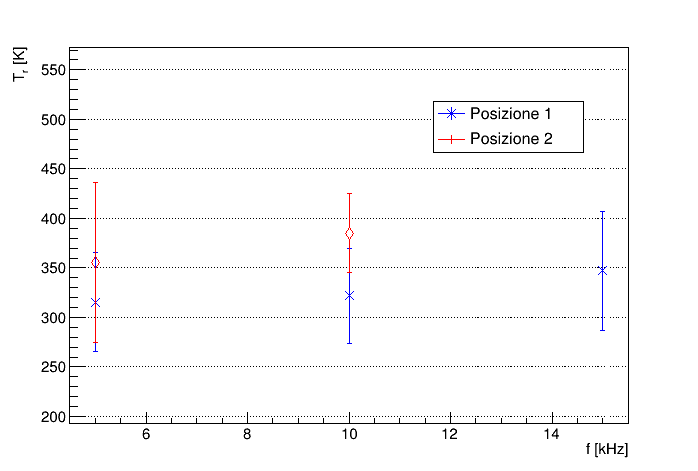
\includegraphics[width=0.65\textwidth]{Images/Spectroscopy/TrN2.png}
 \caption{Estimation of rotational temperature of \ce{N2} molecule, for different frequencies, in blue position 1 in red position 2.}
 \label{fig:TrN2}
\end{figure}


\subsection{Vibrational temperature for \ce{N_2}}
How, boltzmann graph, article.

\begin{figure}
\centering
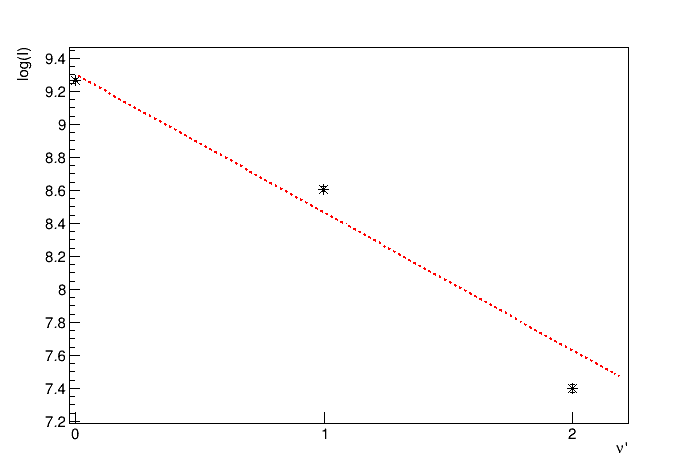
\includegraphics[width=0.65\textwidth]{Images/Spectroscopy/boltzman_f5t16v.png}
 \caption{Example of a boltzmann graph for estimation of vibrational temperature, for low pulse setup and position 1.}
 \label{fig:boltzex}
\end{figure}

\begin{figure}
\centering
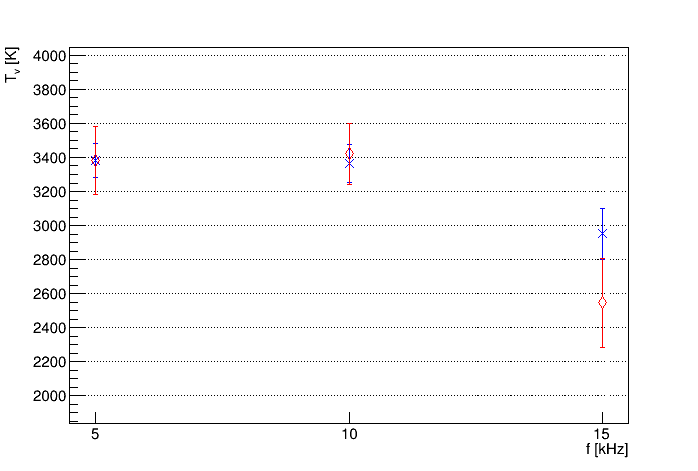
\includegraphics[width=0.65\textwidth]{Images/Spectroscopy/TvN2.png}
 \caption{Estimation of vibrational temperature of \ce{OH} molecule, for different frequencies, in blue position 1 in red position 2.}
 \label{fig:TvN2}
\end{figure}


%Spectrum with different gasses?


\begin{comment}
La determinazione delle specie reattive prodotte dal plasma a pressione atmosferica può essere effettuata tramite misure spettrometriche della sorgente in funzione su un bersaglio.
Gli effetti del trattamento al plasma si pensano dovuti alla presenza di ROS e RNS, quindi vengono raccolte misure nel range di lunghezze d'onda utili ad osservare le emissioni di molecole di \ce{OH} (\SI{305.00}-\SI{313.00}{\nano\meter}), \ce{N_{2}} (\SI{280.00}-\SI{500.00}{\nano\meter}) e \ce{NO} (\SI{220.0}-\SI{290.0}{\nano\meter}) (vedi articoli).

I prototipi di sorgente sviluppati permettono di variare il range dei parametri di funzionamento, in modo da modulare l'intensità del trattamento. Per verificare come cambia lo spettro in base alle diverse modalità di funzionamento, si osservano la variazione nell'intensità delle emissioni al cambiare di frequenza e tempo di apertura del circuito.

Si vuole osservare l'intensità relativa delle righe al variare del gas in ingresso, quindi la sorgente viene azionata con diverse miscele di gas. La misura standard viene effettuata con flusso di \ce{He}, nella solita modalità di funzionamento della sorgente. Vengono poi predisposte due ulteriori modalità di misura dove il gas viene fatto gorgogliare in una soluzione di acqua o di ammoniaca prima dell'inserimento all'uscita della sorgente, per arricchire i prodotti delle reazioni di ioni contenenti, rispettivamente, ossigeno o azoto.

A partire dalla forma delle righe di alcune specie molecolari, è inoltre possibile stimare la temperatura rotazionale alla quale avviene l'emissione misurata. Le emissioni dovute alla molecola \ce{OH} o \ce{N_2} sono varie righe dalle intensità variabili a seconda della temperatura delle molecole, misurando l'intensità relativa dei picchi si può ricavare la temperatura rotazionale delle molecole.

\section{Setup di acquisizione}

Per la sorgente vengono utilizzati sia il prototipo precedente, \textbf{prototipo 1} , sia il prototipo svilupato durante questo lavoro, \textbf{prototipo 2}.

Vengono inoltre provate tre diverse modalità di funzionamento della sorgente, variando frequenza e tempo di chiusura del circuito, mostrate in Tabella \ref{tab:setsorgente}.
Il flusso del gas di elio viene mantenuto pari a \SI{2}{\liter/\minute}.

\begin{table}
 \centering
 \begin{tabular}{cc}
 \toprule
 $f$ [\si{\kilo\hertz}]  &$\Delta t$ [\si{\micro\second}]\\
 \midrule
 5  &15\\
 10 &10\\
 15 &10\\
 \bottomrule
 \end{tabular}
 \caption{Parametri di funzionamento utilizzati per le diverse misure.}
 \label{tab:setsorgente}
\end{table}



\section{Presentazione ed analisi misure}
Per entrambe le sorgenti, l'analisi prevede il riconoscimento delle emissioni misurate, il confronto delle intensità variando distanza e parametri di funzionamento della sorgente, il confronto delle intensità variando il gas immesso, la stima delle temperature rotazionali delle molecole \ce{OH} e \ce{N_2}.

\subsection{Riconoscimento righe}
L'output dello spettrometro viene letto tramite routine IDL ed il riconoscimento dei picchi viene effettuato tramite la classe TSpectrum presente nelle librerie ROOT. Ogni misura viene confrontata con uno spettro di background preso con lo stesso tempo di acquisizione e sorgente spenta, riuscendo così ad escludere i picchi dovuti al fondo.
In figura \ref{fig:spettrotot} si vedono le principali righe estrapolate dalle acquisizioni, in particolare si vedono le righe relative ad \ce{NO}, \ce{OH}, \ce{H_{2}} e \ce{N_{2}}, tabulate in Tabella \ref{tab:spettrotot} .

\begin{figure}
\centering
\includegraphics[width=0.99\textwidth]{Immagini/spettrotot_unico_label_def.png}
\caption{Spettro acquisito con condizioni di misura standard ($f = \SI{5}{\kilo\hertz}$ e $\Delta t = \SI{16}{\micro\second}$), obiettivo puntato vicino l'uscita del gas dalla sorgente.}
\label{fig:app}
\end{figure}


L'acquisizione migliore, nella quale vengono riconosciuti più picchi, è quella mostrata in Figura \ref{fig:spettrotot}, corrispondente alla posizione 1 e condizioni standard di misura, $f = \SI{5}{\kilo\hertz}$.

\paragraph{}
Per verificare gli effetti di una diversa frequenza  nel funzionamento della sorgente vengono confrontate le intensità relative alle righe di \ce{OH} e \ce{N_2}, sommando i conteggi per le varie porzioni di spettro. Non vengono prese in considerazione le righe del gruppo relativo all'\ce{NO} in quanto troppo deboli. In Tabella \ref{tab:irel_1} i risultati, dove vengono confrontate i conteggi alle varie frequenze rispetto i conteggi ottenuti nelle condizioni standard di lavoro, $f = \SI{5}{\kilo\hertz}$. Si nota un calo evidente nei conteggi, crescente con l'aumentare della frequenza di lavoro.

Allo stesso modo viene variata la posizione dell'obbiettivo, dalla posizione 1, puntato all'uscita della sorgente, alla posizione 2, puntato all'uscita del bersaglio. I risultati sempre in Tabella \ref{tab:irel_1}, dove vengono presentati i conteggi nella posizione 2 rispetto i conteggi nella posizione 1. Viene trovato un effetto diverso sulle diverse specie, le emissioni di \ce{OH} diminuiscono molto, mentre quelle relative l'\ce{N_2} diminuiscono in maniera inferiore.

\begin{table}
 \centering
 \begin{tabular}{lcc}
 \toprule
                            &\ce{OH}  &\ce{N_2}\\
 \midrule
 f = \SI{5}{\kilo\hertz}    &1.00     &1.00\\
 f = \SI{10}{\kilo\hertz}    &0.95    &0.81\\
 f = \SI{15}{\kilo\hertz}    &0.62    &0.63\\
 \midrule
 posizione 1                &1.00        &1.00\\
 posizione 2                &0.10     &0.82\\
 \bottomrule
 \end{tabular}
 \caption{Intensità relative delle porzioni interessanti di spettro, al variare di frequenza e posizione, per il prototipo 1.}
 \label{tab:irel_1}
\end{table}


\subsection{\ce{He} + \ce{H_2O} e \ce{He} + \ce{NH_3}}
Vengono misurati gli spettri di emissione in condizioni di lavoro standard, $f = \SI{5}{\kilo\hertz}$, posizione 1, trattando il flusso di elio prima di inserirlo nella sorgente.
Per il prototipo 1, l'arricchimento di specie reattive dell'ossigeno o dell'azoto avviene facendo gorgogliare l'elio in una soluzione di acqua o ammoniaca, mantenendo un flusso in uscita dalla bombola sempre di \SI{2}{\liter/\minute}.
Le misure così acquisite presentano un'intensità molto minore per tutte le righe dello spettro e non vi sono variazioni rilevanti per le lunghezze d'onda interessate, cioè le emissioni relative ad \ce{OH} per la soluzione di acqua e relative ad \ce{N_2} per la soluzione di ammoniaca.

\subsection{Stima temperatura}
Lo spettro di emissione della molecola \ce{OH} è della forma presentata in Equazione \ref{eq:fitOH} (vedi articolo):
\begin{equation}
\centering
\begin{split}
&I_i (T) = I_{0,i} \exp{-\frac{E_n (T-T_0)}{T_0 T}} \\
&S_i(\lambda,T) = \frac{I_i(T)}{\sigma \sqrt{2\pi}} \exp{\frac{(\lambda - \lambda_i)^2}{2\sigma^2}}\\
&S(\lambda,T) = \sum_i S_i(\lambda,T)
\end{split}
\label{eq:fitOH}
\end{equation}

dove $I_i$ è l'intensità ad una determinata energia $E_n$ e $I_{0,i}$ è l'intensità misurata ad una temperatura di riferimento $T_0$. Le $S_i$ sono la convoluzione di $I_i$ con una distribuzione gaussiana nelle $\lambda$ e lo spettro finale $S$ sarà la somma degli spettri relativi la singola transizione.
Simulando diversi spettri nelle varie temperature, sarà possibile stimare la temperatura rotazionale degli ioni presenti nel gas.

La procedura consiste nel simulare diversi spettri $S(\lambda,T)$ come presentati in \ref{eq:fitOH}, calcolare gli scarti quadratici medi rispetto le misure e ricavare la temperatura dalla simulazione migliore. Tipicamente sono stati simulati spettri con $200$ temperature diverse, su un range di temperature possibili variabili, a seconda della misura considerata.
L'errore sulla stima della temperatura viene calcolato come media della differenza tra la temperatura minima che avesse uno scarto quadratico medio fino al $5\%$ superiore rispetto al minimo e la differenza della temperatura massima con le stesse condizioni.

In figura \ref{fig:fitT} sono presentati due esempi di fit delle emissioni interessate. In \ref{tab:Trot} vengono presentate le diverse temperature ottenute, compatibili tra loro.

\begin{figure}
 \centering
 \subfloat[][\ce{OH}]
  {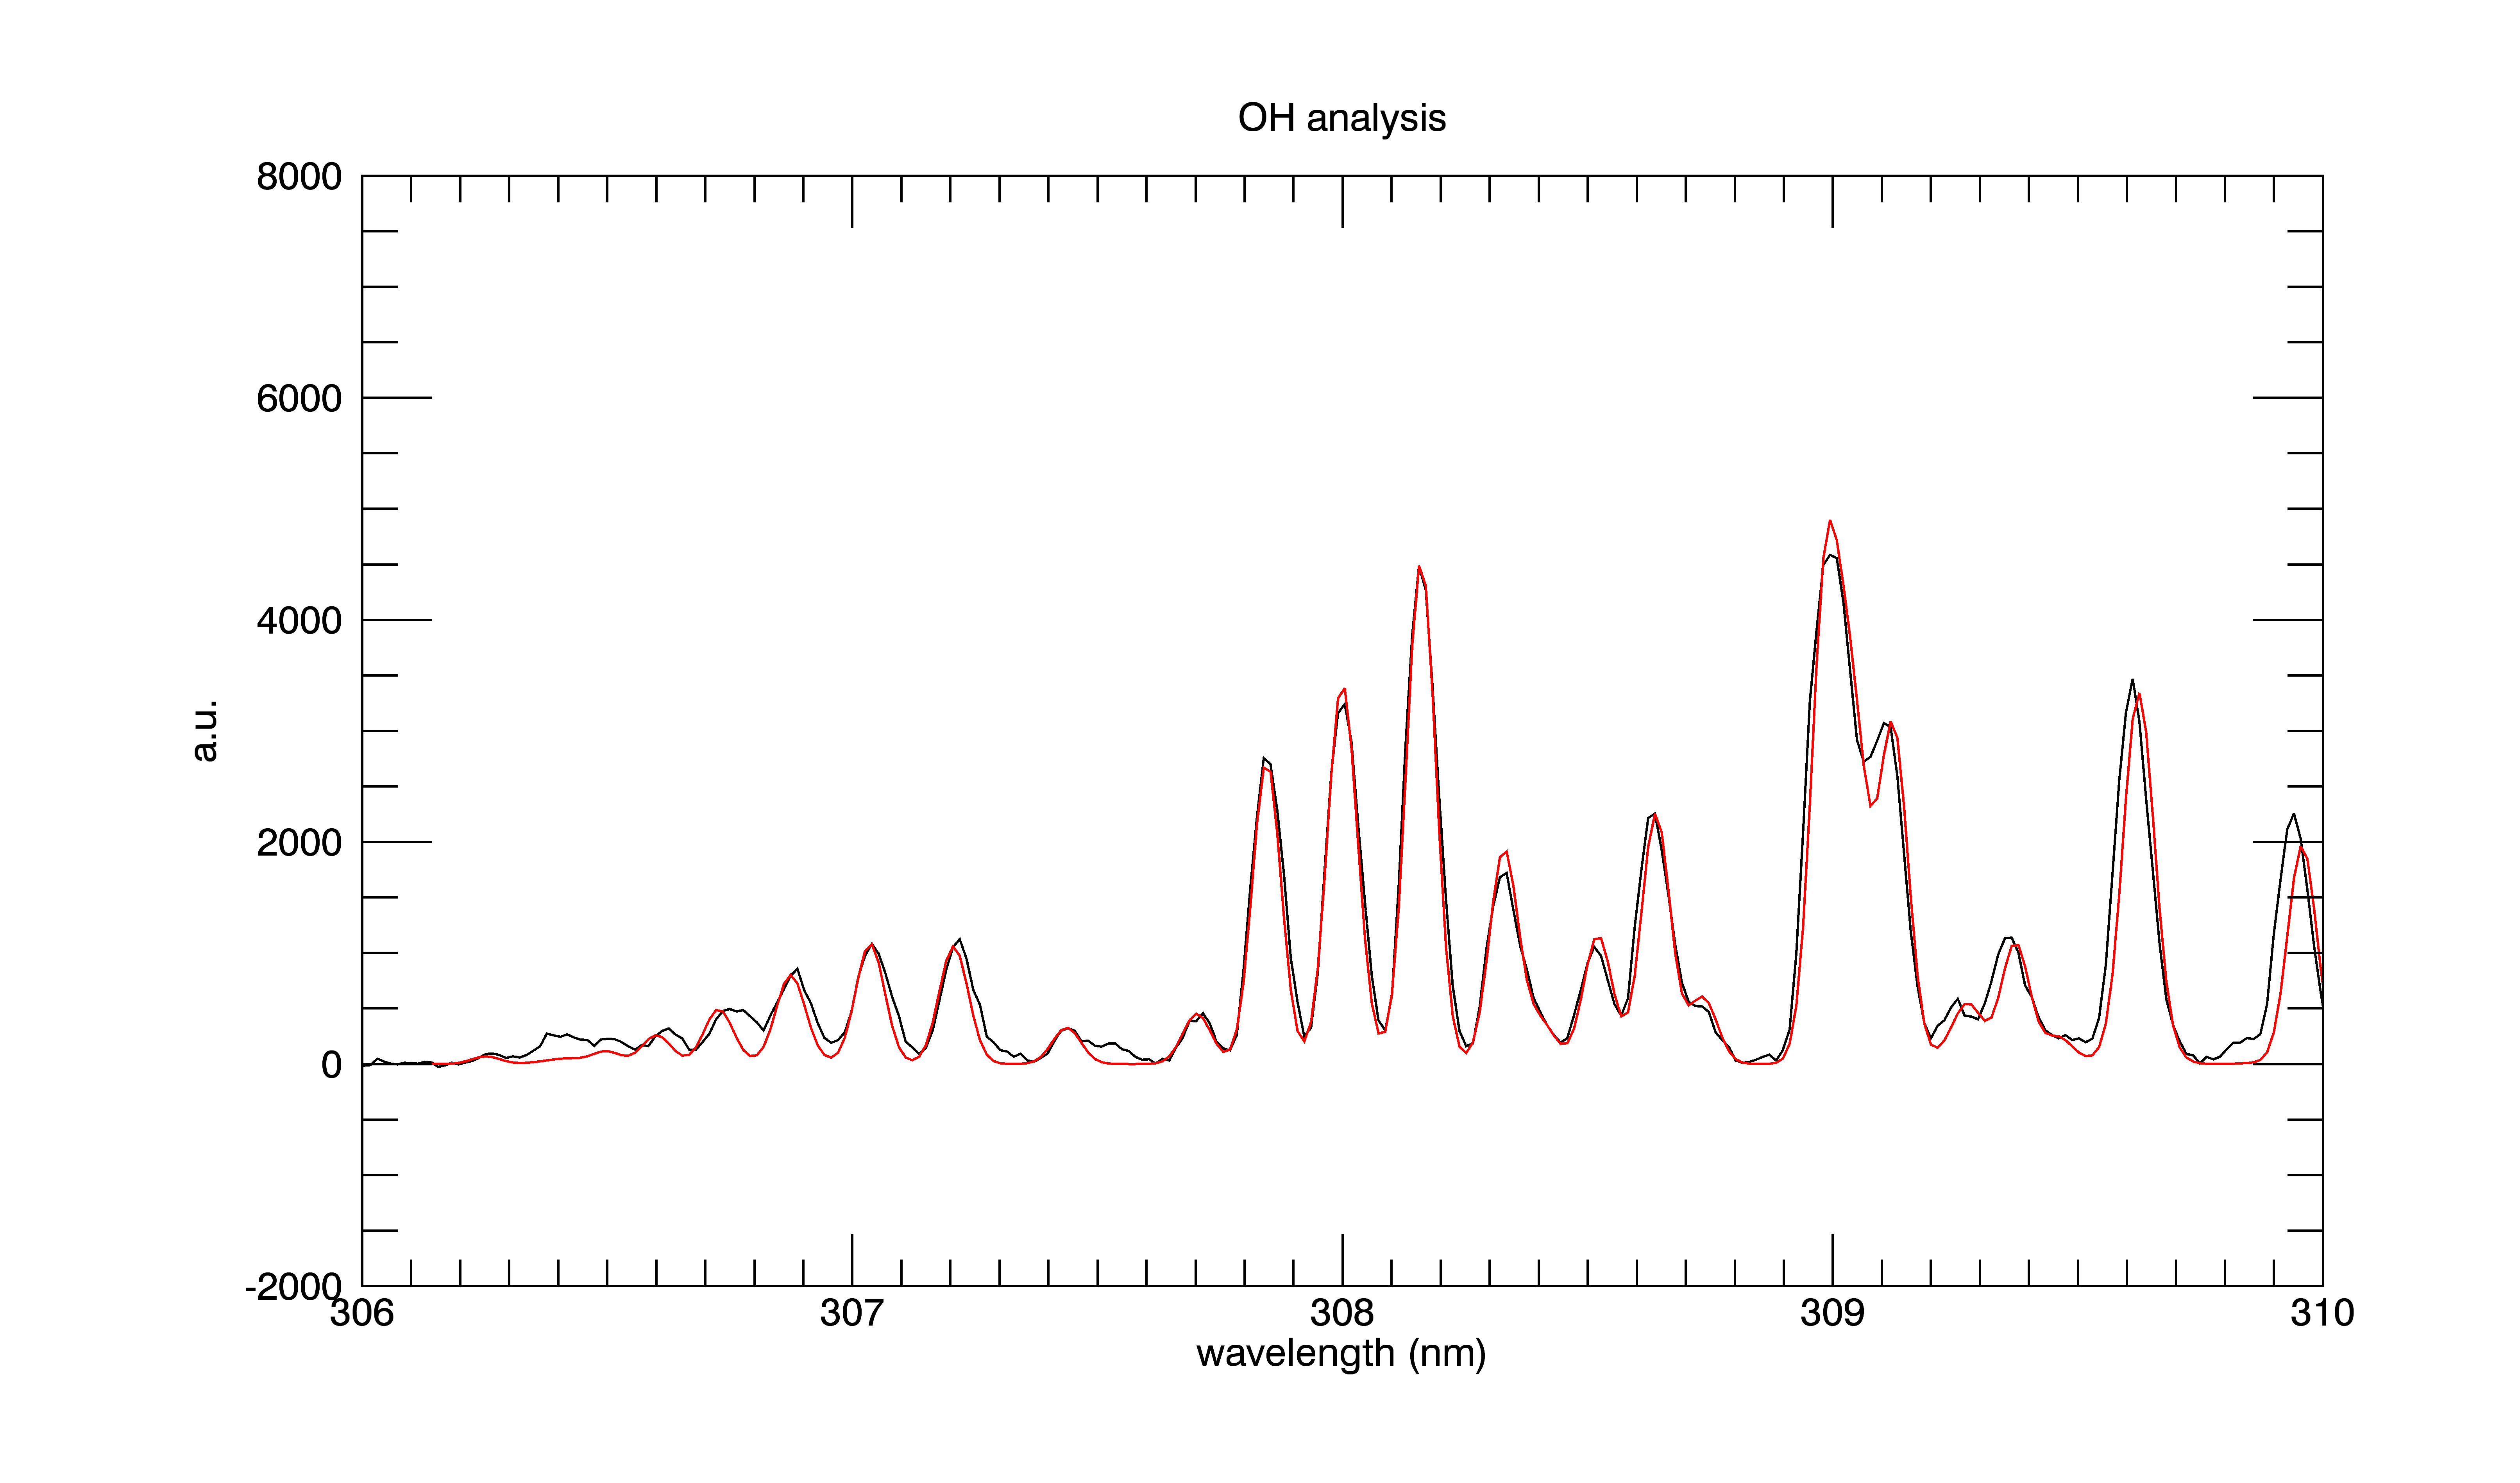
\includegraphics[width=.8\textwidth]{Immagini/OHFit_f5t16elio.png}}
 \\
 \subfloat[][\ce{N_2}]
  {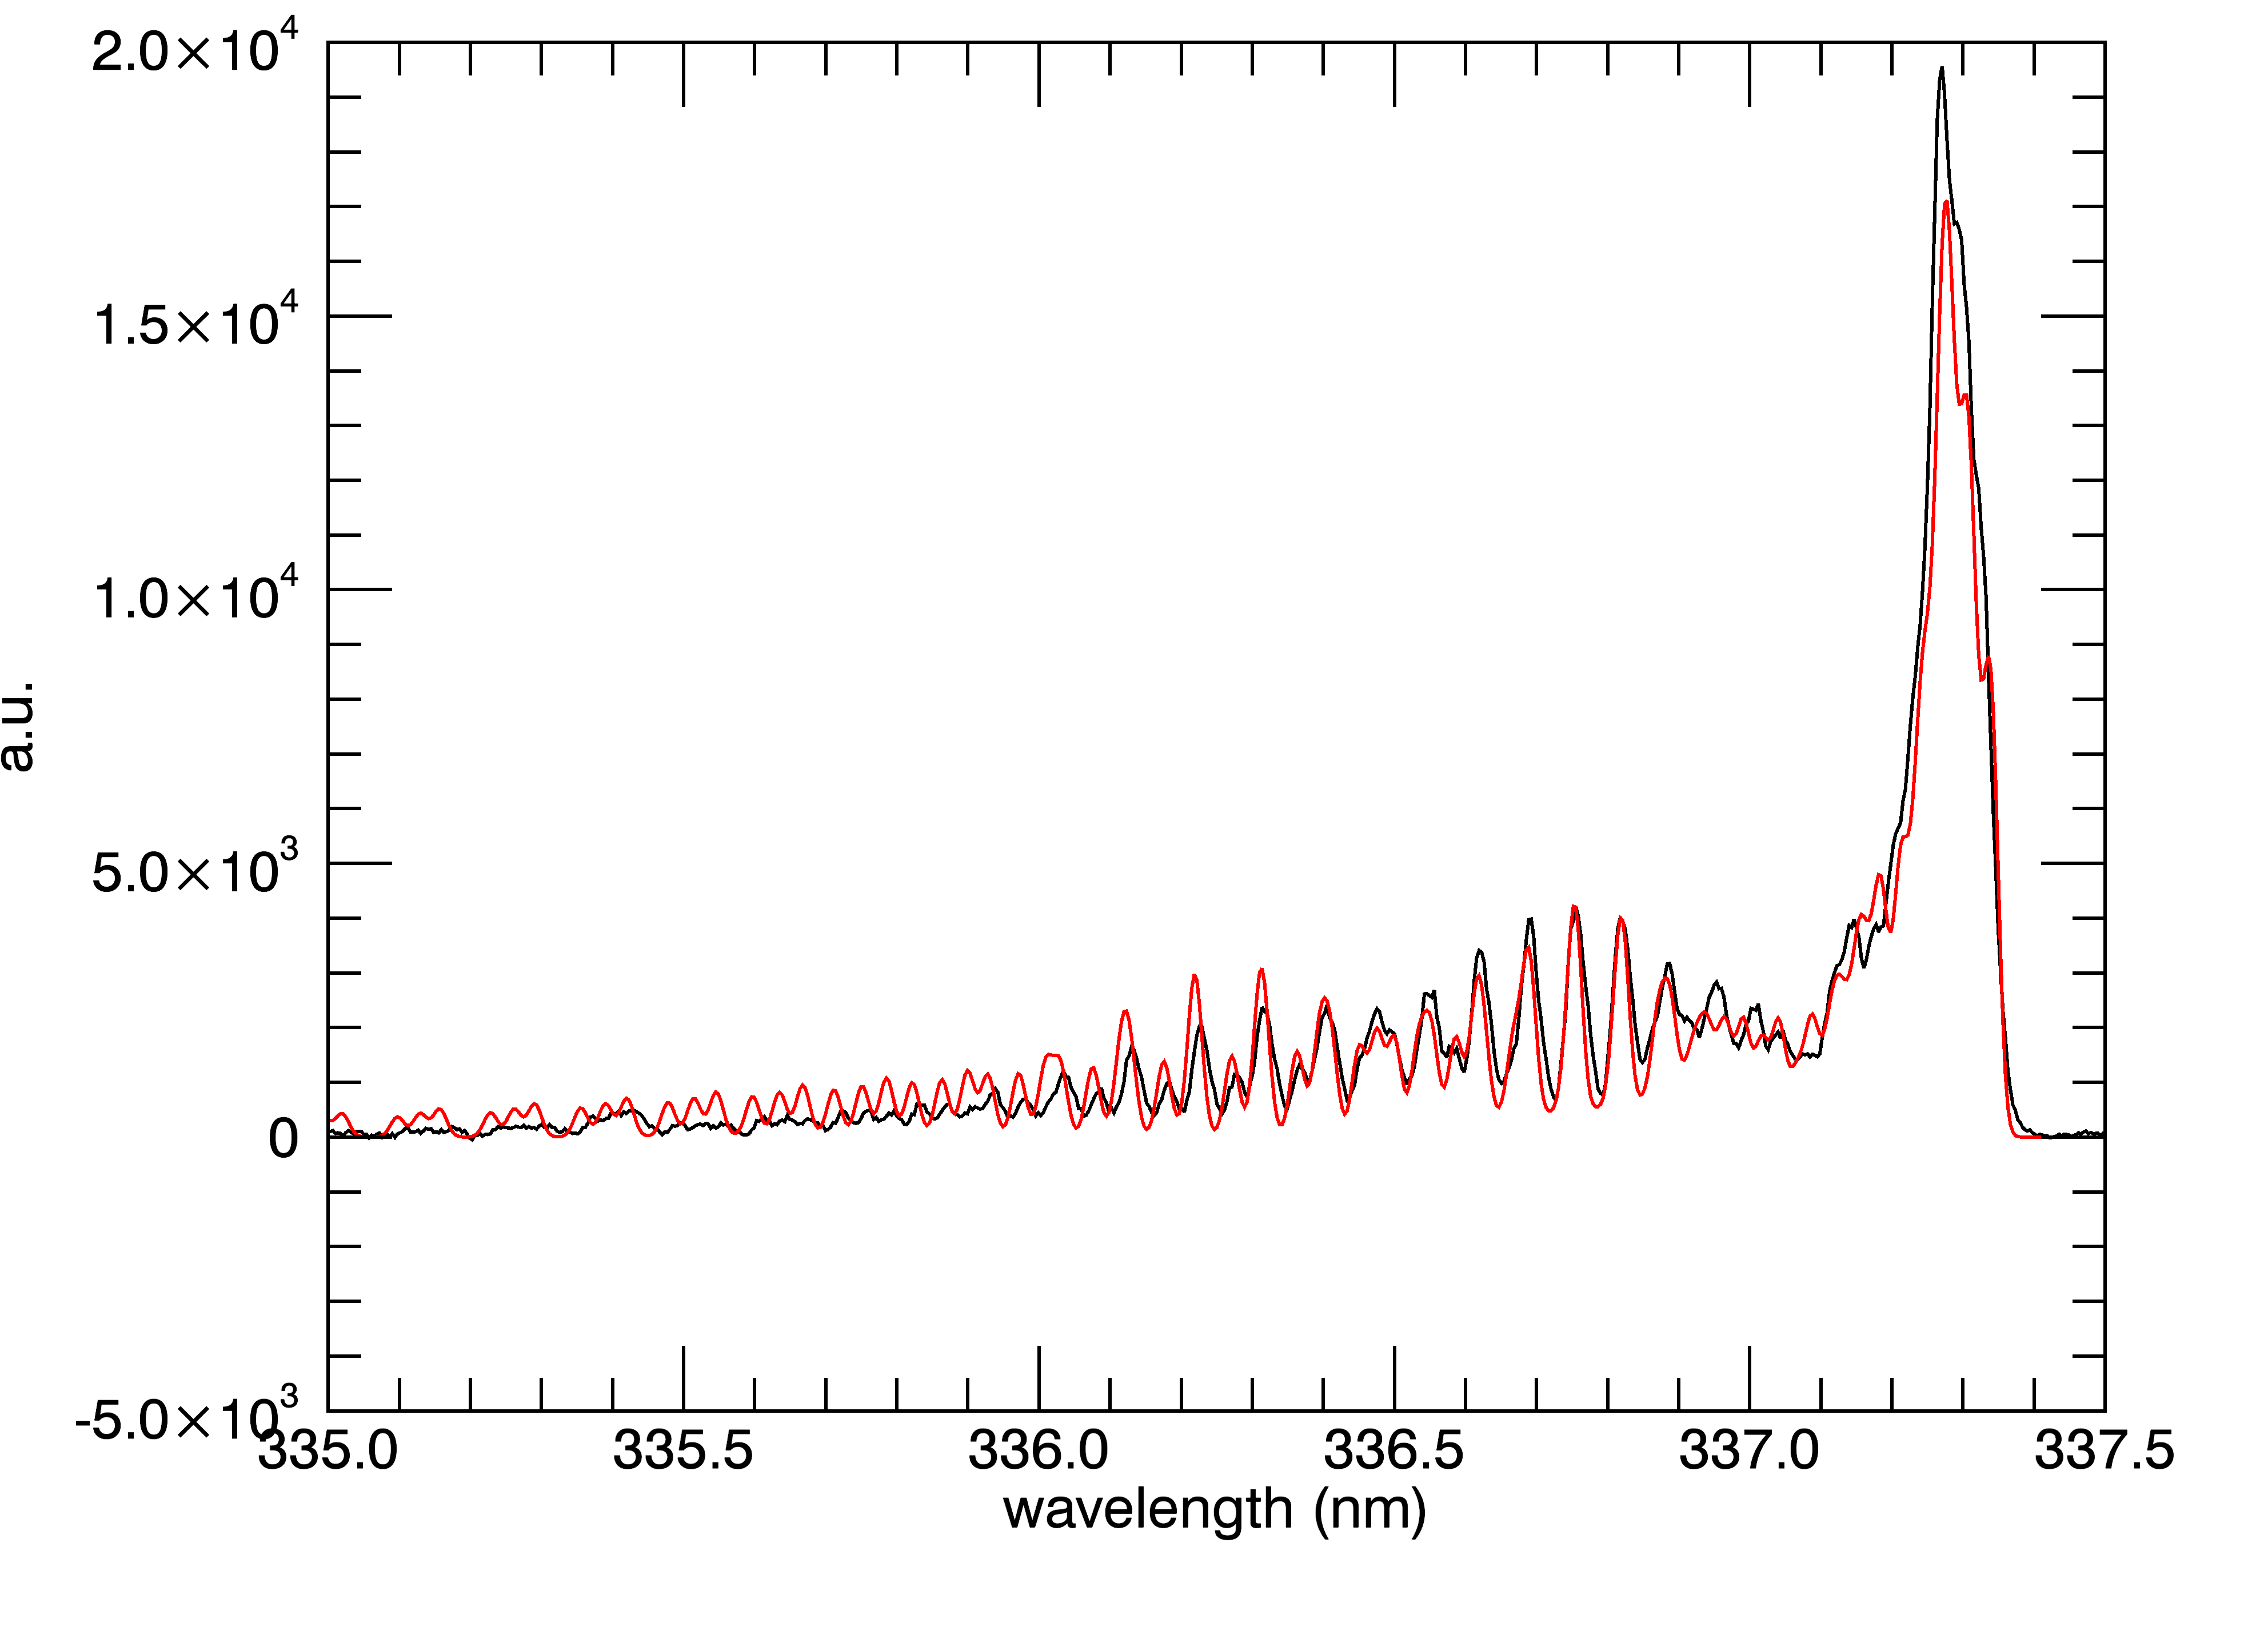
\includegraphics[width=.75\textwidth]{Immagini/N2rotFit_elio.png}}
 \caption{Fit delle emissioni con spettri simulati, misure prese con il prototipo 1, in condizioni standard, posizione 1.}
 \label{fig:fitT}
\end{figure}

\begin{table}
 \centering
 \begin{tabular}{cc}
 \toprule
            &T [\si{\kelvin}]\\
 \midrule
  \ce{OH}   &$336 \pm 30$\\
  \ce{N_2}  &$322 \pm 41$\\
 \bottomrule
 \end{tabular}
 \caption{Stima delle temperature di rotazione delle molecole.}
 \label{tab:Trot}
\end{table}
\end{comment}

\begin{comment}
La misura viene effettuata tramite uno spettrometro IsoPlane dalla lunghezza focale di \SI{320}{\milli\meter}, con tre diversi reticoli: \SI{150}, \SI{1200} e \SI{2400}{g/\milli\meter}, corrispondenti alle risoluzioni di ... .
La risoluzione maggiore viene utilizzata per acquisire le righe \ce{OH} e \ce{N_{2,\text{rot}}}, mentre per acquisire lo spettro totale vengono utilizzati i reticoli a piccola e media risoluzione.

Lo spettrometro è accoppiato ad una telecamera PIXIS di $2048 \times $ ... pixels quadrati dal lato di ... \si{\micro\meter}, con un massimo di \SI{65000} conteggi per il singolo canale.
La luce viene raccolta da una lente in quarzo di focale ... e diametro ... , portata da una fibra ottica dallo spessore di ... e lunghezza di ... e collegata all'entrata dello spettrometro.

Per l'acquisizione viene posizionata la sorgente in funzione a distanza di \SI{1}{\centi\metre} dal bersaglio in metallo (collegato a terra) con l'ottica focalizzata sul flusso di gas, come in foto \ref{fig:app}. Vengono distinte due posizioni dell'ottica:
\begin{itemize}
 \item posizione 1 = obiettivo sull'uscita della sorgente
 \item posizione 2 = obiettivo sul punto di impatto del plasma sulla sorgente, ad \SI{1}{\centi\meter} dall'uscita della sorgente
\end{itemize}
.

\begin{table}
\centering
 \begin{tabular}{ccc}
  \toprule
                            &$\lambda$ \text{[}\si{\nano\meter}\text{]} &\text{I [arb.u.]}\\
  \midrule
  \multirow{4}*{\ce{NO}}    &\num{236.31(24)}  &27\\
                            &\num{237.00(15)}  &26\\
                            &\num{247.02(5)}  &28\\
                            &\num{247.86(12)}  &27\\
  \midrule
  \multirow{2}*{\ce{OH}}    &\num{308.3(1)}  &106\\
                            &\num{309.1(1)}  &113\\
  \midrule
  \multirow{5}*{\ce{N_2}}   &\num{316.03(1)}  &381\\
                            &\num{337.11(1)}  &1000\\
                            &\num{357.77(1)}  &722\\
                            &\num{367.22(20)}  &58\\
                            &\num{371.12(4)}  &172\\
                            &\num{375.66(2)}  &232\\
                            &\num{380.64(2)}  &423\\
  \midrule
  \multirow{2}*{\ce{N_2^+}} &\num{391.50(2)}  &355\\
                            &\num{427.45(2)}  &180\\
  \midrule
  \ce{H_{\alpha}}           &\num{655.96(4)}  &113\\
  \midrule
  \multirow{2}*{\ce{He}}    &\num{586.94(5)}  &122\\
                            &\num{705.56(1)}  &649\\
  \midrule
  \ce{O}                    &\num{776.39(1)}  &393\\
  \bottomrule
 \end{tabular}
 \caption{Picchi rilevanti nello spettro di emissione del prototipo 1, condizioni di misura standard, posizione 1.}
 \label{tab:spettrotot}
\end{table}


Per ogni misura viene stabilito un tempo di acquisizione idoneo ad avere un numero ottimale di eventi, evitando la saturazione dei singoli canali. Una volta stabilito il tempo viene eseguita una misura di fondo, a sorgente spenta, e successivamente viene avviata la misura con sorgente attiva.
\end{comment}
